\documentclass{article}
\usepackage{url}
\usepackage[french]{babel}
\usepackage[T1]{fontenc}
\usepackage[utf8]{inputenc}
\usepackage{graphicx} % Required for inserting images
\usepackage{listingsutf8}
\lstset{%
    inputencoding=utf8,
    literate=
        {é}{{\'e}}{1}%
        {è}{{\`e}}{1}%
        {à}{{\`a}}{1}%
        {â}{{\^a}}{1}%
        {ç}{{\c{c}}}{1}%
        {œ}{{\oe}}{1}%
        {ù}{{\`u}}{1}%
        {É}{{\'E}}{1}%
        {È}{{\`E}}{1}%
        {À}{{\`A}}{1}%
        {Ç}{{\c{C}}}{1}%
        {Œ}{{\OE}}{1}%
        {Ê}{{\^E}}{1}%
        {ê}{{\^e}}{1}%
        {î}{{\^i}}{1}%
        {ï}{{\"i}}{1}%
        {ô}{{\^o}}{1}%
        {û}{{\^u}}{1}%
}
\usepackage{fullpage}
\usepackage{setspace}
\usepackage{todonotes}
\usepackage{amsthm}
\usepackage{amsmath}
\usepackage{amssymb}
\usepackage[all]{xy}

\usepackage[french, frenchkw, boxed, linesnumbered]{algorithm2e}

\newtheoremstyle{exostyle}% style name
{10pt}% above space
{10pt}% below space
{}% body font
{}% indent amount
{\scshape\bfseries\large}% head font
{\hfill\vspace{5pt}\newline}% post head punctuation
{0pt}% Space after theorem head
{\hfill\thmname{#1}\thmnumber{ #2} -- \thmnote{ #3}}% head spec

\newtheoremstyle{partiestyle}% style name
{1em}% above space
{1em}% below space
{}% body font
{}% indent amount
{\bfseries}% head font
{\vspace{.5em}\newline}% post head punctuation
{0em}% Space after theorem head
{\thmnumber{#2} \thmnote{ #3}}% head spec

\newtheoremstyle{questionstyle}% style name
{.5em}% above space
{.5em}% below space
{}% body font
{}% indent amount
{\bfseries}% head font
{}% post head punctuation
{0em}% Space after theorem head
{Question \thmnumber{#2 }}% head spec

\theoremstyle{exostyle}
\newtheorem{exo}{Exercice}

\theoremstyle{partiestyle}
\newtheorem{partie}{}[exo]

\theoremstyle{questionstyle}
\newtheorem{question}{Question}[exo]
\newtheorem{questionpartie}{Question}[partie]

\title{Examen terminal Algorithmie Avancée}
\author{L3 MPCI}
\date{13 janvier 2026 - Durée: 2h}

\begin{document}

\maketitle

\begin{center}
{\em\bf Lorsque l'on vous demande d'écrire de décrire ou de donner un algorithme cela signifiera toujours en donner un pseudo-code, justifier de son exactitude et de sa complexité}

~\\

{\em On rappelle qu'aucun document ni équipement électrique ou électronique n'est autorisé. }
\end{center}

\paragraph*{Les trois exercices sont indépendants ; les deux premiers valent chacun un quart des points totaux.}

\paragraph*{Pour toutes les questions :}
\begin{itemize}
\item les graphes seront considérés non orientés,
\item le nombre de sommets d'un graphe vaudra $n$,
\item le nombre d'arêtes d'un graphe vaudra $m$,
\end{itemize}

\clearpage

\begin{exo}[Méthode probabiliste]
	On va utiliser la méthode probabiliste pour démontrer des résultats sur les problèmes SAT et $k$-SAT.

		Soient $x_1, \dots, x_n$, $n$ variables booléennes. On définit :

	\begin{itemize} 
		\item un {\bf \em littéral } $l$ comme étant soit une variable $l = x_i$, soit sa négation $l = \overline{x_i}$ 
	\item une {\bf \em clause } comme étant une disjonction de littéraux $c = l_1 \lor \dots
\lor l_k$ avec $l_1, \dots l_k$ des littéraux portant sur \underline{$k$ variables différentes}
\item une {\bf \em conjonction de clauses } comme étant $f = c_1\land \dots \land c_m$ (avec $c_1, \dots c_m$ des clauses) \end{itemize}

 Le problème SAT cherche à savoir s'il existe des valeurs pour lesquelles $f$ est vraie. Si tel est le cas,
la conjonction de clauses est dite {\bf \em satisfiable }.
		
	Pour une assignation $x_i = v_i \in \{\text{VRAI}, \text{FAUX}\}$ pour tout $1 \leq i \leq n$ donnée, on dira qu'une clause est {\bf \em satisfaite} si elle est vraie pour cette affectation et on notera $S(f, v_1, \dots, v_n)$ le nombre de clauses de $f$ satisfaites. Enfin on notera $S(f) = (\max S(f, v_1, \dots, v_n))/m$ la proportion maximale de clauses satisfiables (si $f$ est satisfiable alors $S(f) =  1$).
	\begin{partie}[SAT]
	\begin{questionpartie}
		Rappelez les définitions des ensembles NP et NP-complet et pourquoi le problème SAT y est associé.
	\end{questionpartie}
	\begin{questionpartie}
	    Pour une conjonction de $m$ clauses $f$ donnée, que peut-on dire de $S(f, v_1, \dots, v_n) + S(f, \overline{v_1}, \dots, \overline{v_n})$ ?
	\end{questionpartie}
	\begin{questionpartie}
En déduire que $1/2 \leq S(f) \leq 1$ quelque soit $f$. Donnez une conjonction de clause telle que $S(f) = 1/2$.
	\end{questionpartie}
	\begin{questionpartie}
	Donnez un algorithme de complexité linéaire rendant une assignation satisfaisant d'au moins la moitié des clauses d'une conjonction de clauses $f$ passée en paramètre.
		\end{questionpartie}
	\end{partie}
	\begin{partie}[$k$-SAT]
		une $k$-clause est une clause constituée d'exactement $k$ littéraux.
		\begin{questionpartie}
			Pour une affectation aléatoire des variables, quelle est la probabilité qu'une $k$-clause soit non satisfaite ?
		\end{questionpartie}
		\begin{questionpartie}
			En déduire que toute conjonction de $m < 2^k$ $k$-clauses est satisfiable.
		\end{questionpartie}
		\begin{questionpartie}
			Montrez que que pour toute conjonction $f$ de $m$ $k$-clauses on a $S(f)\geq 1-\frac{1}{2^k}$
		\end{questionpartie}
		\begin{questionpartie}
			Conclusions pour une conjonction $f$ de $m$ $3$-clauses ?
		\end{questionpartie}
		
	\end{partie}

% parler de 2-SAT, de 3-SAT et de passer de sat a 3-sat
% monter qu'une conjonction de clause est presque surement satisfiable. Mais rare a trouver.


\end{exo}		
		
\begin{exo}[Graphes]
	% Un graphe $G = (V, E)$ est dit {\em \bf cordé} si pour tout cycle $x_1\dots x_px_1$ il existe $2\leq i + 1 < j \leq p$ tel que $x_ix_j$ soit une arête.
	\begin{question}
		Rappelez la définition de clique et de clique maximale d'un graphe.
	\end{question}
	\begin{question}
		Soit $G = (V, E)$ un graphe connexe et $\mathcal{C}$ l'ensemble de ses cliques maximales. Montrez que si quelque soit $x \in V$ on a $|\{ C \,\vert\, x \in C, C \in \mathcal{C}\}| = 1$ ($x$ n'appartient qu'à une seule clique maximale de $G$), alors $G$ est le graphe complet.
	\end{question}
	\begin{question}
		Soit $G$ un graphe connexe et non complet d'au moins 3 sommets. Montrer qu'il existe un sommet $x$ appartenant à au moins deux cliques maximales différentes.
	\end{question}
	\begin{question}
		Soit $G$ un graphe connexe. Montrer que supprimer un sommet $x$ n'appartenant qu'à une seule clique maximale ne déconnecte pas le graphe.
	\end{question}
	\begin{question}
Donnez un algorithme permettant de savoir si un sommet $x$ donné est dans une seule clique maximale d'un graphe $G$.
	\end{question}

% 	\begin{question}
%  % c'est faux.
% 		Soit $G$ un graphe cordé connexe et non complet. Montrer que pour tout sommet $x$ appartenant à au moins deux cliques maximales différentes, la restriction de $G$ à $V \backslash \{x\}$ n'est pas connexe.
% 	\end{question}
% 	\begin{question}
% 		Montrer que $(i) \Leftrightarrow (ii)$ :
% 		\begin{itemize}
% 			\item[$(i)$] $G$ est cordé
% 			 \item[$(ii)$] 
% 			 \begin{itemize}
% 			 \item il existe un sommet $x$ de $G$ qui n'appartient qu'à une seule clique maximale,
% 			 \item $G$ privé de $x$ est  cordé.
% 			  \end{itemize}
% 		\end{itemize}
% 	\end{question}
% 	\begin{question}
% Donnez un algorithme polynomial  permettant de reconnaître si un graphe est cordé.
% 	\end{question}
\end{exo}

% utiliser la proposition de knuth pour rendre cet algorithme linéaire https://www.youtube.com/watch?v=txaGsawljjA 


\begin{exo}[Enquête policière]
	On doit cet exercice à Claude Berge qui l'a publié en 1994 sous le nom de {\em Qui a tué le duc de Densmore ?} dans le fascicule 67 de la bibliothèque Oulipienne (voir \url{https://iti.mff.cuni.cz/series/2013/598.pdf} p75-90).
	
	\paragraph{Le récit :}
	{\em
		Les huit récits suivants qui relatent des événements précédant le meurtre du duc
		de Densmore (découvert plus d’une année trop tard) ont été recueillis par le détective
		Ralston de Scotland Yard auprès des huit dernières personnes à avoir vu le duc en vie
		(à des moments différents), à savoir :	\\
		\begin{itemize}
		\item Miss {\bf F}elicia Wynn (mannequin rencontrée par le duc à bord du Sam Loyd au cours
		d’une croisière en Méditerranée)
		\item Lady {\bf C}ynthia Mansfield (joueuse professionnelle au casino de Monte-Carlo)
		\item Mrs {\bf G}eorgia Blake (théosophe végétarienne et spirite)
		\item Miss {\bf D}iana Macleod (traductrice du livre de Georges Perec {\em Les Choses})
		\item Miss {\bf E}mily Healey (lépidoptèologiste rousse)
		\item Miss {\bf A}nn Laybourn (joueuse d’échecs avec un ELO à 2075)
		\item Miss {\bf B}etty Townsend (pianiste)
		\item Miss {\bf H}elen Grimshaw (jeune comédienne ayant joué à treize ans le rôle de Zazie à
		Nottingham, et à seize ans celui de Vittoria dans Le Démon Blanc de Webster)
		\end{itemize}
	    En raison de 1’ancienneté des événements, ces huit personnes n’ont pu se rappeler
		les dates exactes de leurs séjours respectifs chez le duc, et les récits qui s’y rapportent
		ne figurent donc pas ici dans l’ordre chronologique.
	}
	\paragraph{[ ... ]}
		\paragraph{didascalie}{Vous lirez la nouvelle en entier pour vous imprégner de l'histoire ce soir, mais pour que tout cela tienne dans le temps de l'examen, je résume.}
	
	Le duc est mort dans l'explosion de son manoir et votre mission est de trouver l'assassin, en sachant que :
	\begin{itemize}
		\item L'assassin est une des 8 femmes
		\item Chaque personne n'est venue qu'une seule fois au château
		\item Aucune autre personne n'est venue au château
		\item Pendant leur séjour au château :
	\begin{itemize}
	\item A a rencontré B, C, E, F, et G
	\item B a rencontré A, C, et H
	\item C a rencontré A, B, D, E, et H
	\item D a rencontré C, et E
	\item E a rencontré A, C, D, et F
	\item F a rencontré A, et E
	\item G a rencontré A, et H
	\item H a rencontré B, C, et G
	\end{itemize}
	\item L'assassin a dû se cacher pour fabriquer la bombe : pendant qu'elle était cachée elle n'a rencontré personne et personne n'a pu la voir.
	\end{itemize}
	\begin{partie}[Étude préliminaire]
		\begin{questionpartie}
			\label{q1}
			Représentez les relations de rencontre entre les 8 femmes par un graphe dont les sommets sont les 8 femmes et les arêtes les rencontres.
		\end{questionpartie}
		\begin{questionpartie}
			Montrer que que si personne ne s'était caché on pourrait retrouver ce graphe en connaissant les dates d'arrivée et de départ de chacune des 8 femmes.
		\end{questionpartie}
		\begin{questionpartie}
			Qu'en déduire pour du graphe de rencontre de la question~\ref{q1} ?
		\end{questionpartie}
	\end{partie}
	\begin{partie}[Graphes d'intervalles]

Si $I_1, \dots I_n$ sont $n$ intervalles fermés de $\mathbb{R}$, on appelle graphe d'intersection de ces intervalles le graphe $G=(V, E)$ où :

		\begin{itemize}
			\item $V = \{I_1, \dots, I_n\}$
			\item $xy \in E$ si $x \cap y \neq \varnothing$
		\end{itemize}
		
		On appelle {\bf \em graphe d'intervalles} un graphe $G=(V, E)$ pour lequel il existe $n$ intervalles fermés de $\mathbb{R}$ tels que $G$ soit son graphe d'intersection.
				    \begin{figure}[h]
			    \centering
		\begin{minipage}{.45\textwidth}
		\centering
			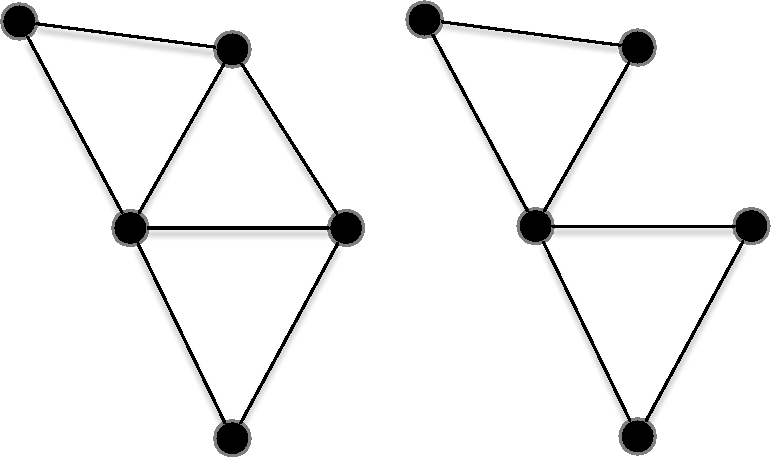
\includegraphics[scale=0.2]{fig2.pdf}
			\caption{Deux graphes d'intervalles connexes\label{fig2}} 
		\end{minipage}
		\begin{minipage}{.45\textwidth}
		\centering
			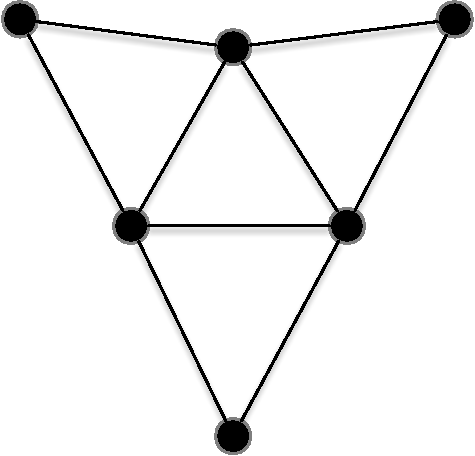
\includegraphics[scale=0.2]{3-sun.pdf}
			\caption{Un graphe interdit\label{3-sun}} 
		\end{minipage}
	\end{figure}

		\begin{questionpartie}
			Donnez les graphes d'intervalles associées à :
			    \begin{itemize}
			    \item $V = \{ [1, 5], [1, 4], [3, 7], [6, 10]\}$
			    \item $V = \{ [1, 5], [1, 4], [3, 7], [5, 10]\}$
			    \end{itemize}
		\end{questionpartie}
		\begin{questionpartie}
			Donnez des intervalles associés aux deux graphes connexes de la figure~\ref{fig2} et montrez qu'il peut y avoir plusieurs solutions.
		\end{questionpartie}
				\begin{questionpartie}
			Montrez que les graphes complets et discrets sont des graphes d'intervalles
		\end{questionpartie}
				\begin{questionpartie}
			Montrez que si $G=(V, E)$ est un graphe d'intervalles alors la restriction de $G$ à $V'$ est un graphe d'intervalles pour tout $V' \subseteq V$.
		\end{questionpartie}

		\begin{questionpartie}
			Montrez que les cycles sans corde (il n'existe aucune autre arête que celles du cycle) de strictement plus de 3 arêtes ne peuvent être des graphes d'intervalles.\label{q2}
		\end{questionpartie}
		\begin{questionpartie}
			\label{q3}
			Montrez que le graphe de la figure~\ref{3-sun} ne peut pas être un graphe d'intervalles.
		\end{questionpartie}
	\end{partie}
	\begin{partie}[Résolution de l'énigme]
		\begin{questionpartie}
			Montrez que le graphe de la question~\ref{q1} n'est pas un graphe d'intervalles.
		\end{questionpartie}
		\begin{questionpartie}
			Explicitez pourquoi en supprimant l'assassin du graphe de la question~\ref{q1} on obtient un graphe d'intervalles. En déduire une procédure permettant de terminer l'assassin.
		\end{questionpartie}
		\begin{questionpartie}
			En utilisant les questions~\ref{q2} et~\ref{q3} déterminez la personne qui s'est cachée, {\em ie.} l'assassin.
		\end{questionpartie}
		\begin{questionpartie}
		\label{q4}
			Puisque seul l'assassin a menti, reconstituez un graphe d'intersection possible. Montrez qu'il peut y en avoir plusieurs. Combien de fois au minimum l'assassin s'est-il caché ?
			\end{questionpartie}
			\begin{questionpartie}
			En utilisant votre graphe de la question~\ref{q4} représentez une solution possible pour les intervalles de présence des 8 femmes. Y en-a-t-il plusieurs possibles ?
		\end{questionpartie}

	% faire le théorème complet de reconnaissance.
	\end{partie}

\end{exo}

\end{document}
